\documentclass[11pt, aspectratio=1610]{beamer}
\usetheme{Boadilla}
\usepackage[utf8]{inputenc}
\usepackage{amsmath}
\usepackage{amsfonts}
\usepackage{amssymb}
%\author{}
\title{Extract an unknown function in a non-parametric way}
%\setbeamercovered{transparent} 
%\setbeamertemplate{navigation symbols}{} 
%\logo{} 
%\institute{} 
%\date{} 
%\subject{} 
\newcommand{\bfy}{\mathbf{y}}
\newcommand{\bfye}{\mathbf{y}^{\textrm{exp}}}
\newcommand{\dbfye}{\delta\mathbf{y}^{\textrm{exp}} }
\newcommand{\like}{ \textrm{Likelihood}}
\newcommand{\prior}{ \textrm{Prior}}
\begin{document}

\begin{frame}
\titlepage
\end{frame}

\begin{frame}
\tableofcontents
\end{frame}
\section{The standard Bayes approach already contains the ``sequential'' calibration of parameters.}
\begin{frame}{The standard Bayes approach}
Suppose the following dependence of two sets of observables $y$ on parameters $x$.
\begin{itemize}
\item $\bfy_1=\bfy_1(x_1)$ only depends on $x_1$.
\item $\bfy_2=\bfy_2(x_1,x_2)$ depends on both $x_1$, $x_2$.
\end{itemize}

Suppose, people have measured $\bfy_1$ long ago in the past: 
$\bfye_1 \pm \dbfye_1$, and then someone used it to extract information of $x_1$,
\begin{eqnarray}
\nonumber
P_1(x_1) = {\color{orange}\prior(x_1)\like\left( \frac{\bfy_1(x_1)-\bfye_1}{\dbfye_1}\right)}
\end{eqnarray}

Few years later,$\bfye_2 \pm \dbfye_2$ are measured, but we don't want to vary $x_1$ arbitrarily when extracting $x_2$, so we use $P_1(x_1)$ as informative prior:
\begin{eqnarray}
\nonumber
P_{12}(x_1, x_2) &=& P_1(x_1)\prior(x_2)\like\left( \frac{\bfy_2(x_1,x_2)-\bfye_2}{\dbfye_2}\right)\\\nonumber
&=& {\color{orange}\prior(x_1)}\prior(x_2){\color{orange}\like\left( \frac{\bfy_2(x_1,x_2)-\bfye_2}{\dbfye_2}\right)}\like\left( \frac{\bfy_1(x_1)-\bfye_1}{\dbfye_1}\right)
\end{eqnarray}
{\bf The same as calibrated to both dataset simultaneously.}
\end{frame}

\section{To avoid data sensitive to low-$T$ constrains parameter at high-$T$ requires better functional parametrization}
\begin{frame}{The subtly is in the parametrization of unknown functionals}
For example,  usually, we try temperature dependence of $\hat{q}$
\begin{eqnarray}
\nonumber
\frac{\hat{q}}{T^3} = A+B\left(\frac{T}{T_c}\right)^C
\end{eqnarray}
The problem: $A, B$, and $C$ controls the temperature dependence in a highly correlated manner $\rightarrow$ May leads to correlated change of all parameters when we include new dataset.
{\vskip 1em}
Step-function like parameterization
\begin{eqnarray}
\nonumber
\frac{\hat{q}}{T^3} = a_0(1\sim 1.5 T_c) + a_1(1.5\sim 2 T_c)+ a_2(2\sim 2.5 T_c)+ a_3(2.5\sim 3 T_c)+ a_4(3\sim 4 T_c)
\end{eqnarray}
Decorrelate from one temperature to another. Potential problem: lack of adjacent correlation:
\begin{columns}
\begin{column}{.3\textwidth}
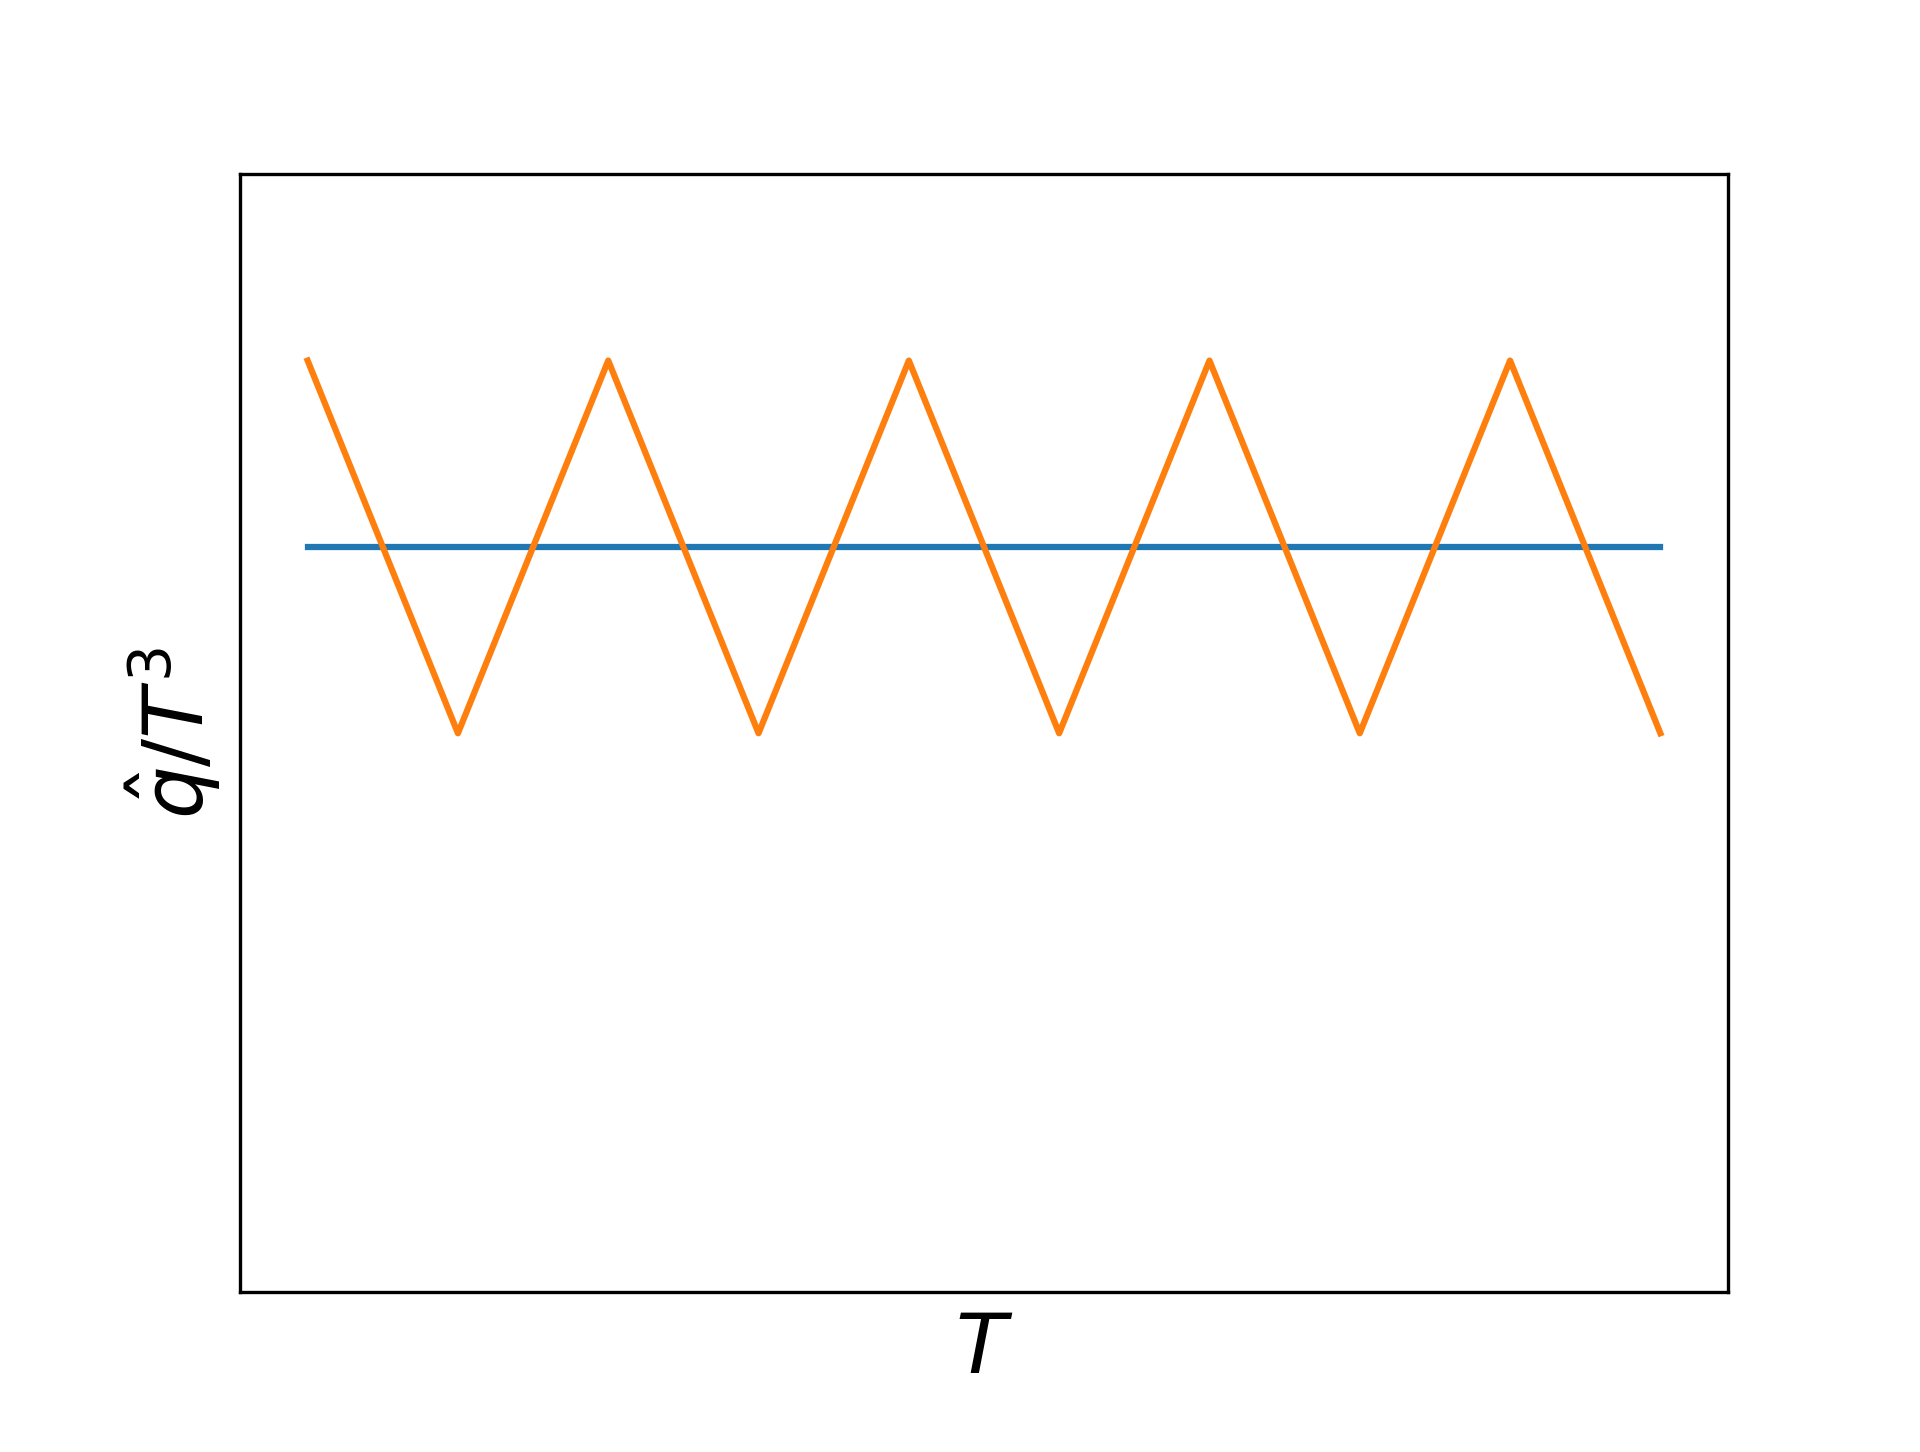
\includegraphics[width=\textwidth]{step.png}
\end{column}
\begin{column}{.7\textwidth}
To avoid the yellow case, we can manipulate the choice of prior in a correlated way! Not long range correlation, but finite-range correlation that $P_0(x \rightarrow x_1) = P_1(x_1)$.
$\rightarrow$ no need to change the model computation procedure, just need a carefully designed prior.
\end{column}
\end{columns}
\end{frame}

\section{A non-parametric way to parametrize the unknown functional of $\hat{q}(T)$.}
\begin{frame}{A proposed way to parametrize unknown functional form of $\hat{q}/T^3$}
\begin{itemize}
\item Treat $\hat{q}/T^3$ as some unknown function in a functional space that:
\begin{itemize}
\item If I know $\hat{q}/T^3$ at low temperature, I am still agnostic to its high-$T$ behavior.
\item If I know $\hat{q}/T^3$ at $T_1$, its value at adjacent temperature must be close to the value at $T_1$.
\end{itemize}
\item Easily modeled by a random function sampled by the Gaussian process.
\begin{eqnarray}
\nonumber
P[\hat{q}(T)] \sim \mathcal{GP}\left(\textrm{mean}=\hat{q}_0, \textrm{cov}=C e^{-\frac{(\ln T-\ln T')^2}{2\sigma^2 } } \right)
\end{eqnarray}
\end{itemize}
\begin{columns}
\begin{column}{.4\textwidth}
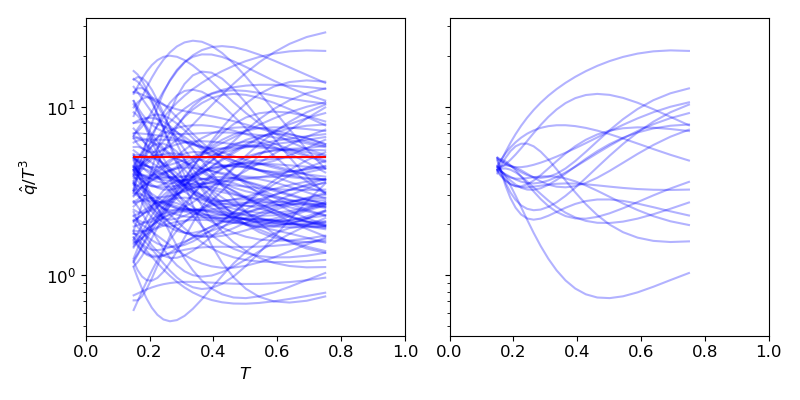
\includegraphics[width=\textwidth]{qhat_sample.png}
\end{column}
\begin{column}{.6\textwidth}
``Infinitely'' many points, but effectively only $\frac{\ln(T_{\max}/T_{\min})}{\sigma}$ d.o.f.. A smooth version of ``independently vary'' $\hat{q}$ at temperature far apart with short-range correlation. 
\\
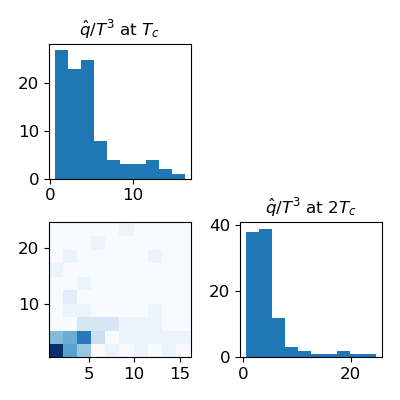
\includegraphics[width=.4\textwidth]{qhat_long.png}
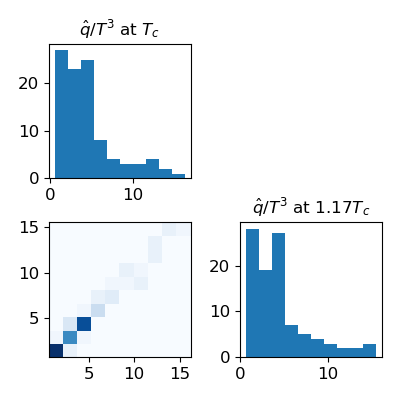
\includegraphics[width=.4\textwidth]{qhat_short.png}
\end{column}
\end{columns}
\end{frame}

\begin{frame}{Workflow}
Run physical model:
\begin{itemize}
\item Generate, e.g. 100,  realization of $P[\hat{q}(T)]$.
\item Model predictions: centrality, energy, collision system, $p_T$ dependent.
\end{itemize}
The following jobs is purely statistical.
\begin{itemize}
\item The fact that the parameterization $\hat{q}(T)$ is uncorrelated from $\hat{q}(T')$ if $T$ and $T'$ are sufficently different prevents low-$T$-sensitive data from constraining high-$T$ parameters.
\item Use emulators to learn the mapping from $\hat{q}(T_i, i=1,2,3\cdots)$ to observables.
\item Using Bayes theorem to get the posterior distribution of $\hat{q}$:
\begin{eqnarray}
\nonumber
P(\hat{q}[T]) = \int D[\hat{q}(T)] P_{\mathcal{GP}}[\hat{q}(T)] \like(\frac{\bfy_{\textrm{emulator} }[\hat{q}(T)]-\bfye}{\dbfye})
\end{eqnarray}
\end{itemize}
{\bf A non-parametric way to extract $\hat{q}(T)$}\\
{\bf I do not know any application like this before in literature. We may need to use a ``toy'' model to evaluate its performance before using real model.
}
\end{frame}

\end{document}
